\documentclass{article}
\usepackage{style}
\usepackage{ctex}
\usepackage[ruled, linesnumbered, algo2e]{algorithm2e}
\usepackage{graphics,graphicx,epstopdf}
\usepackage{amsmath, amsfonts, amsthm}

\usepackage{graphicx, epstopdf}
\usepackage{color}
\usepackage{cite}
\usepackage{indentfirst}
\usepackage{geometry, graphicx}
\usepackage[title]{appendix}
\usepackage{algorithm, algorithmic}
\usepackage{bm}
\usepackage[hidelinks]{hyperref}
\usepackage{multirow}
\usepackage{ulem}
\geometry{left = 5em, right = 5em}
\usepackage{listings}
\usepackage{xcolor}
%% notation macro
\newcommand{\F}{\mathcal F}
\newcommand{\T}{\mathcal T}
\newcommand{\I}{\mathcal I}
\newcommand{\U}{\mathcal U}
\newcommand{\R}{\mathbb R}
\renewcommand{\P}{\mathcal P}
\newcommand{\uP}{ \mathcal \uline P}
\newcommand{\B}{\mathcal B}
%\newcommand{\R}{\mathbb R^2}
\newcommand{\Z}{\mathbb Z}
\newcommand{\C}{\mathbb C}
\newcommand{\laplacian}{\triangle}
\newcommand{\grad}{\nabla}
\renewcommand{\div}{\textrm{div~}}

\newcommand{\diff}[2]{\frac{\partial #1}{\partial #2}}
\newcommand{\difff}[3]{\frac{\parial #1^2}{\partial #2 \partial #3}}
\newcommand{\diFF}[2]{\frac{\partial #1^2}{\partial^2 #2}}
\newcommand{\diam}{\text{ diam }}
%% non-noation macro
\newcommand{\IN}{\text{  in  }}
\newcommand{\ON}{\text{  on  }}
\newcommand{\st}{\text{s.t.  }}
\newcommand{\tbc}{{\color{red}[TBC]}}
\newcommand\ldq\textquotedblleft
\newcommand\rdq\textquotedblright{}
\newcommand\mb\mathbb
\newcommand\mf\mathbf
\newcommand\tf\textbf

\newcommand{\return}{\textbf{return~}}
\DeclareMathOperator{\argmin}{arg~min}
%% enviorment
\newtheorem{proposition}{Proposition}
\newtheorem{definition}{Definition}
\newtheorem{corollary}{Corollary}
\newtheorem{remark}{Remark}


\setlength{\parindent}{1.5em}
\definecolor{mygreen}{rgb}{0,0.6,0}
\definecolor{mygray}{rgb}{0.5,0.5,0.5}
\definecolor{mymauve}{rgb}{0.58,0,0.82}
\lstset{ %
	backgroundcolor=\color{white},      % choose the background color
	basicstyle=\footnotesize\ttfamily,  % size of fonts used for the code
	columns=fullflexible,
	tabsize=4,
	breaklines=true,               % automatic line breaking only at whitespace
	captionpos=b,                  % sets the caption-position to bottom
	commentstyle=\color{green},  % comment style
	escapeinside={\%*}{*)},        % if you want to add LaTeX within your code
	keywordstyle=\color{blue},     % keyword style
	stringstyle=\color{mymauve}\ttfamily,  % string literal style
	frame=single,
	rulesepcolor=\color{red!20!green!20!blue!20},
	% identifierstyle=\color{red},
	language=matlab,
	numbers=left,
}

\makeatletter
\newenvironment{breakablealgorithm}
{% \begin{breakablealgorithm}
		\begin{center}
			\refstepcounter{algorithm}% New algorithm
			\hrule height.8pt depth0pt \kern2pt% \@fs@pre for \@fs@ruled
			\renewcommand{\caption}[2][\relax]{% Make a new \caption
				{\raggedright\textbf{\ALG@name~\thealgorithm} ##2\par}%
				\ifx\relax##1\relax % #1 is \relax
				\addcontentsline{loa}{algorithm}{\protect\numberline{\thealgorithm}##2}%
				\else % #1 is not \relax
				\addcontentsline{loa}{algorithm}{\protect\numberline{\thealgorithm}##1}%
				\fi
				\kern2pt\hrule\kern2pt
			}
		}{% \end{breakablealgorithm}
		\kern2pt\hrule\relax% \@fs@post for \@fs@ruled
	\end{center}
}
\makeatother

%\lhead{\textbf {\showtopic} }
%\chead{} 
%\rhead{\textbf {\showabs} }
%\lfoot{} 
%\cfoot{\thepage}
%\rfoot{} 
%\renewcommand{\headrulewidth}{0.4pt} 
\newtheorem{假设}{假设}
\newcommand{\ui}{u(i*(N+2)^2+j*(N+2)+k)}
\newcommand{\mO}{\mathcal O}
\title{并行与分布式计算上机作业2}
\date{\today}	
\author{
	敖睿成 1900012179\\
	数学科学学院\\
	\texttt{archer\_arc@pku.edu.cn} \\
}
\begin{document}

	\maketitle
	\thispagestyle{fancy}
	\tableofcontents
	\section{摘要}
考虑在$\Omega=[0,1]\times[0,1]\times[0,1]$ 上的Poisson方程:
\begin{equation}\label{eq1}
	\left\{\begin{array}{rr}
		-\Delta u(x, y, z)=f(x, y, z), & (x, y, z) \in \Omega \\
		u(x, y, z)=0, & (x, y, z) \in \partial \Omega
	\end{array}\right.
\end{equation}
其中心差分离散格式可以写为
\begin{equation}\label{eq2}
\left\{\begin{aligned}
	6 U_{i, j, k}-U_{i-1, j, k}-U_{i+1, j, k}-U_{i, j-1, k}-U_{i, j+1, k}-U_{i, j, k-1}-U_{i, j, k+1}=h^{2} f_{i, j, k}, & 1 \leq i, j, k \leq N \\
	U_{0, j, k}=U_{N+1, j, k}=U_{i, 0, k}=U_{i, N+1, k}=U_{i, j, 0}=U_{i, j, N+1}=0, & 0 \leq i, j, k \leq N+1
\end{aligned}\right.
\end{equation}
其中三边被$(N+1)$等分,$h$为网格步长$1/(N+1)$,$U_{i,j,k} = u(ih,jh,kh)$。在本次上机作业中,我们在古典的Jacobi迭代和Gauss-Seidel迭代的基础上,通过去除或改变部分变量之间的依赖关系,给出便于并行的迭代格式,通过MPI,OpenMP和CUDA来数值求解,并作出相应的理论分析。
\begin{figure}[H]
	\centering
	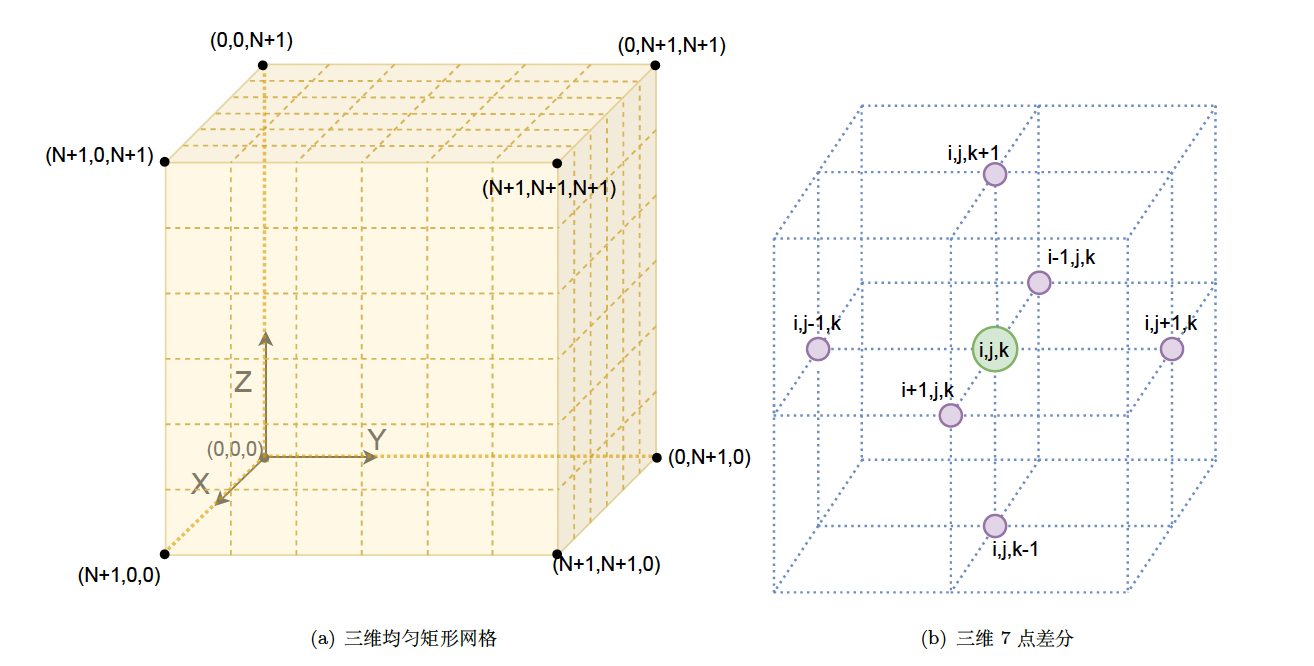
\includegraphics[width=18cm]{./fig/poisson}
	\caption{网格及差分格式}
\end{figure}
\section{算法描述}
在本节,我们给出这次上机作业中用到的算法并分析其性质。在分析过程中,我们假设下面几个条件成立:
\begin{假设}\label{assump1}
原方程的解$U_{i,j,k}$以及其它三维变量的存储格式为形如$u(i*(N+2)^2+j*(N+2)+k)$的一维数组。使用CPU单次访问内存时间为$Tc_{1}$,之后访问连续地址每次所需时间为$Tc_{2}<Tc_{1}$,读了该地址的数据后若下一个命令是再在该地址写入,也只耗费$Tc_{2}$。使用GPU单次访问全局内存时间为$30Tg_{1}$,共享内存与常量内存$5Tg_{1}$,私有内存$Tg_{1}$,同一线程簇中,触发合并访存,访问连续地址的时间分别为$30Tg_{2},5Tg_{2},Tg_{2}$,其中$Tg_{1}>Tg_{2}$。此外,我们假设同一设备的单次计算时间是相同的,分别为$Tc_{3},Tg_{3}$。不同的进程、线程执行相同的命令所需要的时间相同,没有等待时间(除非执行不同的命令或发生了线程簇分歧)。在每一步迭代中,每一个点都被更新恰一次。
\end{假设}
\subsection{Gauss-Seidel迭代}
Gauss-Seidel \cite{seidel1873ueber} 相当于每步求解关于$U_{i,j,k}^*,1\le i,j,k\le N$的线性方程组:
\begin{equation}
	\left\{\begin{aligned}
		6 U_{i, j, k}^{*}-U_{i-1, j, k}^{*}-U_{i+1, j, k}-U_{i, j-1, k}^{*}-U_{i, j+1, k}-U_{i, j, k-1}^{*}-U_{i, j, k+1}=h^{2} f_{i, j, k}, & 1 \leq i, j, k \leq N \\
		U_{0, j, k}^{*}=U_{N+1, j, k}^{*}=U_{i, 0, k}^{*}=U_{i, N+1, k}^{*}=U_{i, j, 0}^{*}=U_{i, j, N+1}^{*}=0, & 0 \leq i, j, k \leq N+1 \\
		U_{0, j, k}=U_{N+1, j, k}=U_{i, 0, k}=U_{i, N+1, k}=U_{i, j, 0}=U_{i, j, N+1}=0, & 0 \leq i, j, k \leq N+1
	\end{aligned}\right.
\end{equation}
实际操作过程中,我们按照$i=1,2,\dots,N,j=1,2,\dots,N,k=1,2,\dots,N$的顺序依次更新$U_{i,j,k}$。但其更新难以并行,采用单核CPU计算,首次访问$u((i+1)*(N+2)^2+(j+1)*(N+2)+1)$及$b(i*N^2+j*N)$时需各$Tc_1$,假定之后访问同一$z$轴上的值均为连续访存,时间为$Tc_2<Tc_1$,而访问$x,y$坐标不同的数据需要$Tc_1$,可以计算单步迭代总时间开销约为$[(4N^3 + N^2) + N^2]Tc_1 + [(2N^3+N^3-N^2)+ N^3-N^2]Tc_2 + 7N^3Tc_3 $,单步残差计算的总时间开销约为$[(4N^3 + N^2) + N^2]Tc_1 + [(2N^3+N^3-N^2)+ N^3-N^2]Tc_2 + 10N^3Tc_3 $。结合两者,得到总时间约为 $\mO((8N^3Tc_1+8N^3Tc_2+17N^3Tc_3)\times Ite)$, 其中$Ite$为总迭代次数。可以看到,串行运行的G-S迭代法所需时间长,且残差计算和迭代过程难以合并,不利于快速计算。
%\begin{figure}
%\centering
%\subfigure{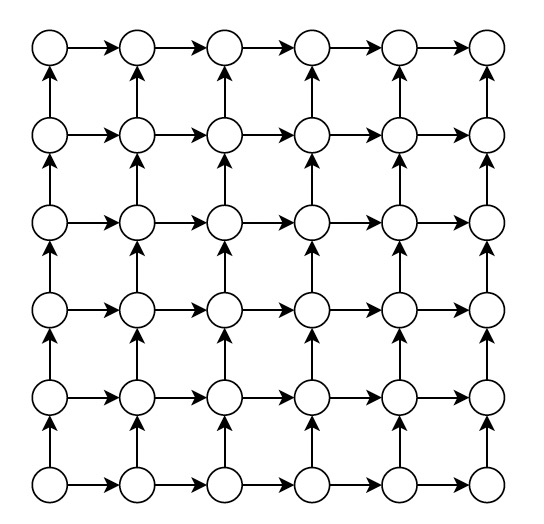
\includegraphics[width=6cm\textwidth]{./fig/gs}}
%\subfigure{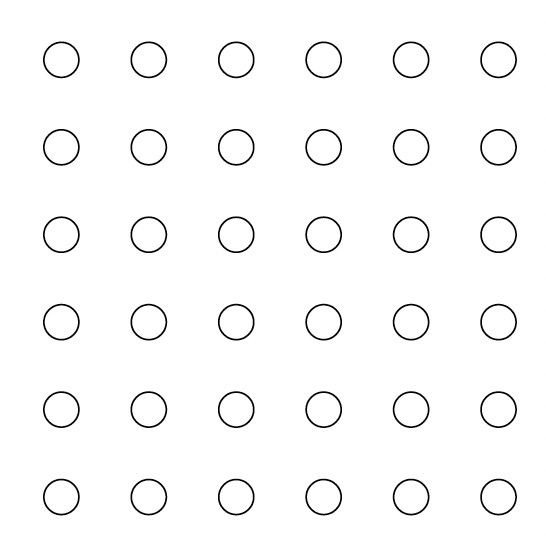
\includegraphics[width=6cm\textwidth]{./fig/jacobi}}
%\caption{Gauss-Seidel和Jacobi迭代}
%\end{figure}
\begin{figure}[H]
	\begin{minipage}[b]{1\linewidth}
		\centering
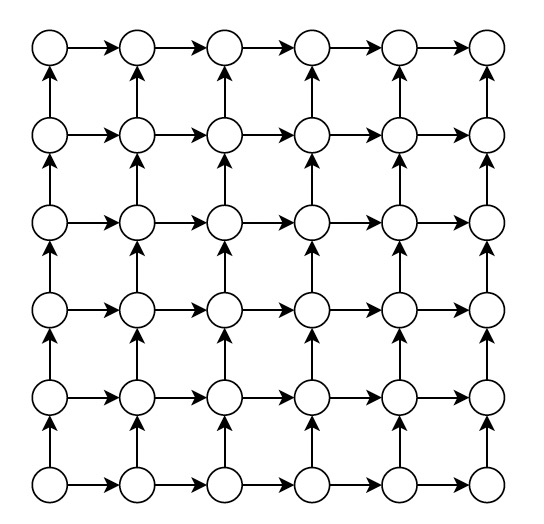
\includegraphics[width=6cm\textwidth]{./fig/gs}
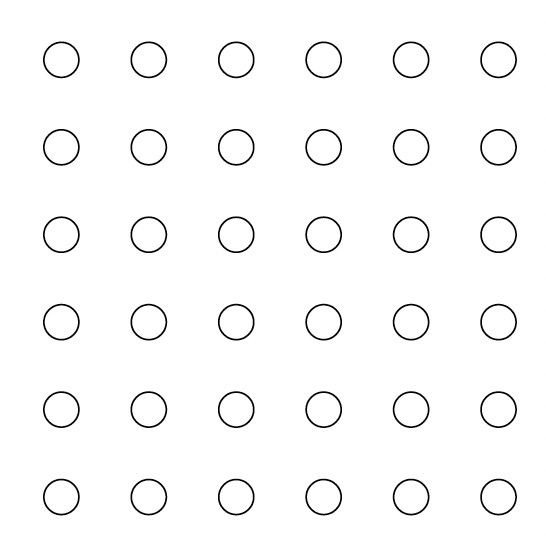
\includegraphics[width=6cm\textwidth]{./fig/jacobi}
	\end{minipage}
\caption{Gauss-Seidel和Jacobi迭代}
\end{figure}

\subsection{Jacobi迭代\label{sec:2.2}}
Jacobi迭代是求解严格对角占优线性方程组的一种方法\cite{golub1996matrix},在实际操作过程中,相当于消除了单步中所有数据之间的依赖关系,也即在第$n$步,令$U_{i,j,k}^n = (b_{i,j,k}+U_{i,j,k-1}^{n-1}+U_{i,j,k+1}^{n-1}+U_{i,j-1,k}^{n-1}+U_{i,j+1,k}^{n-1}+U_{i-1,j,k}^{n-1}+U_{i+1,j,k}^{n-1})/6$,这样的好处是计算过程几乎可以完全并行。采用串行单CPU计算,可以得到单步时间和G-S迭代相同,。如果采用MPI多进程计算,进程数为$Np$,为了尽可能地多进行数据的连续访存,假设我们将每列$z$轴上的元素都看成一个整体,对$Oxy$进行连续地均匀划分成$p$份,每步中每个进程独立计算各自的更新,在每步迭代结尾进行栅栏同步,并且把边界(假定相邻两个部分公共面积为$N^2$)上的数据发送给相邻的两个进程(通信)。假设$MPI$单边通信长为$N^2$的数据需要时间$N^2Tm_1+Tm_2$,那么单步所需要的时间开销约为$(8N^3Tc_1+8N^3Tc_2+17N^3Tc_3)/Np + 2(Np-1)N^2(Tm_1+Tm_2)$。进一步地,可以把计算残差和更新的过程合并,即
\begin{equation}
\left\{\begin{aligned}
	&Res= b_{i,j,k}+U_{i,j,k-1}^{n-1}+U_{i,j,k+1}^{n-1}+U_{i,j-1,k}^{n-1}+U_{i,j+1,k}^{n-1}+U_{i-1,j,k}^{n-1}+U_{i+1,j,k}^{n-1}-6U_{i,j,k}^{n-1},\\
&U_{i,j,k}^n = (b_{i,j,k}+U_{i,j,k-1}^{n-1}+U_{i,j,k+1}^{n-1}+U_{i,j-1,k}^{n-1}+U_{i,j+1,k}^{n-1}+U_{i-1,j,k}^{n-1}+U_{i+1,j,k}^{n-1})/6,
\end{aligned}\right.
\end{equation}
\begin{equation}\label{alg1}
\longrightarrow \left\{\begin{aligned}
&Tmp = b_{i,j,k}+U_{i,j,k-1}^{n-1}+U_{i,j,k+1}^{n-1}+U_{i,j-1,k}^{n-1}+U_{i,j+1,k}^{n-1}+U_{i-1,j,k}^{n-1}+U_{i+1,j,k}^{n-1},\\
&Res = Tmp-6*U_{i,j,k}^{n-1},\\
&U_{i,j,k}^n = Tmp/6,
\end{aligned}
\right.
\end{equation}
其中$Res$是残差,$Tmp$为局部变量。这样做的好处是几乎省掉了一半的计算和访存,缺点是会多计算一次迭代,但实际上,这次迭代的额外计算量只需要一步计算和一次变量$U$的访存,因此在迭代次数较大的时候,该方法在时间上有显著优势,计入了残差规约后,总时间约为$\mO([((4N^3Tc_1 + 6N^3Tc_2+10Tc_3)/Np)+2(Np-1)N^2(Tm_1+Tm_2) ]*(Ite+1) + N^3Tm_3)$,其中$N^3Tm_3$为最后把各部分的解规约到一个进程所需的时间。

对于OpenMP,也能够进行类似的计算,只不过不再有显式的通信时间,而是访存共享变量,隐式同步和循环调度所需要额外的时间。我们用带了$\prime$上标的变量表示访存共享变量所需要的时间,假设用上面类似地使用多线程计算,线程数为$Nt$,并且数组$u$以共享变量的方式存储。这样得到总时间约为$\mO([((4N^3Tc_1^\prime + 6N^3Tc_2^\prime +10Tc_3)/Nt) + N^2 Ts ]*(Ite+1) )$,其中$N^2Ts$为调度循环所需要的时间(我们依然假设以$z$轴一列为一个单位)。我们也可以MPI和OpenMP混合使用来提高并行效率,这里为节省篇幅,不进一步地进行分析。

在GPU上实现Jacobi迭代需要尤其注意访存的开销,我们在允许的范围内尽可能地避免冲突访存,多使用共享内存。基于以上两点,我们一共提出两种实现方式,它们都在迭代过程中用一个线程对应一个格点进行访存、计算。
\begin{itemize}
\item[(a)]对于每一个大小为$L_x\times L_y\times L_z$的block其中的每一个线程$(tx,ty,tz)$,它直接读取对应的格$(x,y,z)$和周围的6个点,通过 \eqref{alg1} 中的方式进行迭代,即在迭代和得到每一格的残差过程中不使用共享内存,但在对残差进行规约时,我们会用到共享内存,在之后会对此进行详细说明。
\item[(b)]对于每一个大小为$L_x\times L_y\times L_z$的block,我们使用大小为$(L_x+2)\times(L_y+2)\times(L_z+2)$大小的共享内存进行扩展,将上一步的数据直接读进共享内存,以对全局内存同一位置的访问进行合并,其余的部分和(a)都相同。
\end{itemize}
这两种方法各有优劣,(a)的好处在于可以节省共享内存的使用,并且避免了(b)在写共享内存时可能造成的conflict和分歧。事实上,注意到在同一个block中,我们只有$L_x\times L_y\times L_z$个线程,而扩展后的$(L_x+2)\times(L_y+2)\times(L_z+2)$不一定是它的倍数,因此可能会发生线程簇分歧的情况,而且实际上在边上的数据是多余的。简要计算可以得到,一次迭代(不包含规约)中,(a)大约需要$30*(4Tg_1+6Tg_2) + Tg_1+2Tg_2$的访存时间(残差也需要使用全局内存中的数组存储,$Tg_1+2Tg_2$为局部变量$Tmp$的访存时间,我们假定连续几步访问同一地址会减少时间),而(b)需要大约$30*((L_x+2)\times(L_y+2)\times(L_z+2))/(L_x\times L_y\times L_z)Tg_2+5*(4Tg_1+3Tg_2) + (30 * 3Tg_2+ Tg_1+2Tg_2)$,这里我们采用的是尽量避免写入冲突的写入共享内存方法。第一项是写入共享内存的开销,第二项是 \eqref{alg1} 中前两行的读共享内存开销,第三项是 \eqref{alg1} 中写入残差,读$b$和更新$u$到全局内存所需要的开销(我们假定触发了合并访存使得残差的写入也是$Tg_2$)。可以看到,理论上block的三个维数越大,第二种方法就越有优势,但实际上维数变大之后,会引起更多if判断越界语句造成的线程簇分歧,而且扩展的数组占用了更多的共享内存,也读入了更多多余的数,因此在我们block大小不超过1024的实验中,(b)的表现不如(a),即简单访存。这两种方法的计算量是相同的,单次迭代中一个线程需要$9Tg_3$的时间计算。此外,我们对残差$Res$进行规约,规约的算法描述如下。
\begin{algorithm}[H]
	\caption{Reduce}
	\begin{algorithmic}[1]
		\STATE{Initial data $a[size]$}
		\STATE{Create shared $d\_a[size]$, $d\_a[tid]=a[tid]$}
		\FOR{$i = (size+1)/2;i > 32;i>>$=$1$}
		\IF{$tid<i$}
		\STATE{$d\_a[tid] += d\_a[tid+i]$}
		\STATE{syncthreads()}
		\ENDIF
		\ENDFOR
		\IF{$tid<32$}
		\STATE{InReduce($d\_a,tid$)}
		\ENDIF
		\IF{$tid = 0$}
		\STATE{Output $d\_a[tid]$}
		\ENDIF
	\end{algorithmic}
\end{algorithm}
其中InReduce是如下用来减少线程簇分歧的函数
\begin{algorithm}[H]
	\caption{InReduce}
	\begin{algorithmic}[1]
\STATE{Input $d_a[size],tid$}
\FOR{$i = 1;i<=32;i*=2$}
\STATE{$d\_a[tid]+=d\_a[tid+i]$}
\ENDFOR
	\end{algorithmic}
\end{algorithm}
可以算得对于大小为$Size$的数组,规约所需的时间大约为$\log_2(size)(Tg_3+2*5Tg_2)+30(Tg_2+Tg_1)$。因此,若记block单次可以让$Ng$个线程同时计算(即$Ng/32$为最大活跃线程簇数,我们假定每个线程计算执行相同命令的计算、访存时间相同,在迭代过程中和Host间的数据拷贝时间可以忽略不计(根据我们具体的实现的确如此),那么使用CUDA的Jacobi迭代需要的总时间约为(a)$\mO([30*(4Tg_1+6Tg_2) + (Tg_1+2Tg_2) + 9Tg_3 + (\log_2(blocksize)*(Tg_3+2*5Tg_2)+30(Tg_2+Tg_1)+10Tg_2)+(\log_2(N^3/blocksize)*(Tg_3+2*5Tg_2)+30(Tg_2+Tg_1) +10Tg_2)]*N^3/Ng * (Ite+1)$,(b)$\mO([30*((L_x+2)\times(L_y+2)\times(L_z+2))/(L_x\times L_y\times L_z)+10Tg_2+5*(4Tg_1+3Tg_2) + (30 * 3Tg_2+ Tg_1+2Tg_2)+ 9Tg_3 + (\log_2(blocksize)(Tg_3+2*5Tg_2)+30(Tg_2+Tg_1)+10Tg_2)+(\log_2(N^3/blocksize)*(Tg_3+2*5Tg_2)+30(Tg_2+Tg_1)+10Tg_2)]*N^3/Ng * (Ite+1))$。可以看到,在$Ng $远大于$Np,Nt$即MPI,OpenMP的进程/线程数时,CUDA计算在时间上具有显著的优势,如下表。
\begin{table}[H]
\begin{tabular}{|c|c|}
	\hline
    Method & Time \\\hline
    MPI &      $\mO([((4N^3Tc_1 + 6N^3Tc_2+10Tc_3)/Np)+2(Np-1)N^2(Tm_1+Tm_2) ]*(Ite+1) + N^3Tm_3)$         \\\hline
    OpenMP &    $\mO([((4N^3Tc_1^\prime + 6N^3Tc_2^\prime +10Tc_3)/Nt) + N^2 Ts ]*(Ite+1) )$         \\\hline
   \multirow{2}*{CUDA} & $\mO([30*(4Tg_1+6Tg_2) + Tg_1+2Tg_2 + 9Tg_3 + \log_2(blocksize) *(Tg_3+2*5Tg_2)+30(Tg_2+Tg_1)$\\& $+10Tg_2+ \log_2(N^3/blocksize)*(Tg_3+2*5Tg_2)+30(Tg_2+Tg_1)+10Tg_2]*N^3/Ng * (Ite+1)$\\
   	\hline
\end{tabular}
	\caption{Jacobi迭代中不同并行方法所需理论时间\label{tb1}}
\end{table}
\subsection{Red \& Black}
红黑着色是依赖关系仅强于Jacobi迭代的一种迭代格式,它可以描述如下。
\begin{algorithm}[H]
	\caption{Red \& Black}
	\begin{algorithmic}[1]
		\STATE{Input $U,b$}
		\WHILE{Not converge}
		\IF{$i+j+k\%2 = 0$ }
		\STATE{$U_{i,j,k}^n = (b_{i,j,k}+U_{i,j,k-1}^{n-1}+U_{i,j,k+1}^{n-1}+U_{i,j-1,k}^{n-1}+U_{i,j+1,k}^{n-1}+U_{i-1,j,k}^{n-1}+U_{i+1,j,k}^{n-1})/6$}
		\ENDIF 
		\STATE{Synchronize}
		\IF{$i+j+k\%2 = 1$ }
		\STATE{$U_{i,j,k}^n = (b_{i,j,k}+U_{i,j,k-1}^{n}+U_{i,j,k+1}^{n}+U_{i,j-1,k}^{n}+U_{i,j+1,k}^{n}+U_{i-1,j,k}^{n}+U_{i+1,j,k}^{n})/6$}
		\ENDIF
		\ENDWHILE
	\end{algorithmic}
\end{algorithm}
\begin{figure}[H]

\centering
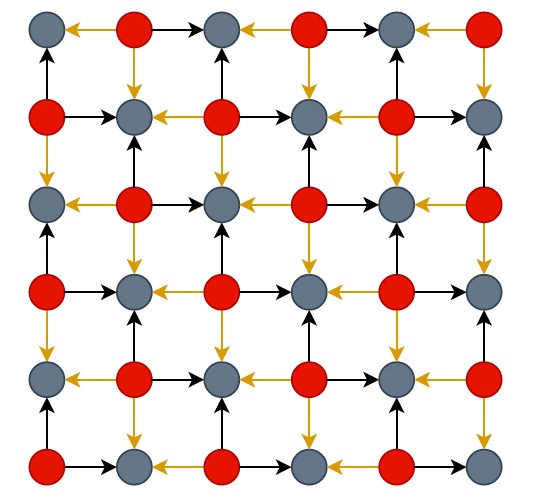
\includegraphics[width=6cm]{./fig/rb}
\caption{Red \& Black\label{fig:rb}}
\end{figure}
相当于奇偶格交错地更新,它可以像之前Jacobi迭代一样高度并行。在MPI和OpenMP上,我们可以按照和Jacobi迭代一样的分块和并行方式,只是把迭代分成两步来做,在CUDA上也是类似的,但在这里需要注意两点。第一,根据我们的残差计算公式,RB每步中后更新的部分实际上残差为0,即每次迭代只需要计算一半的残差,并且可以像\eqref{alg1}里一样和迭代更新进行合并,得到上一步的残差,尽管这样会导致多迭代一次,但同样可以节省约$1/4$的计算和访存,且此时奇数号不需要中间变量$Tmp$。第二,注意到我们的访存实际上是不连续的,实际上,由图 \ref{fig:rb} 立刻可以知道地址间隔至少为2,因此我们可以采用“空间换时间的方法”,即构造两个只有原来一半大小的新数组,让“红格子”和“黑格子”分别放在两个数组中,这样两个数组在计算中地址都是连续的。类似地我们计算得总时间约如下表(CUDA取(a)方案)
\begin{table}[H]
	\begin{tabular}{|c|c|}
		\hline
		Method & Time \\\hline
		MPI &     $\mO([((4N^3Tc_1 + 5N^3Tc_2+9Tc_3)/Np)+2(Np-1)N^2(Tm_1+Tm_2) ]*(Ite+1) + N^3Tm_3)$          \\\hline
		OpenMP &    $\mO([((4N^3Tc_1^\prime + 5N^3Tc_2^\prime +9Tc_3)/Nt) + N^2 Ts ]*(Ite+1) )$         \\\hline
		\multirow{2}*{CUDA} & $\mO([30*(4Tg_1+5Tg_2) + Tg_1+2Tg_2 + 8Tg_3 + \log_2(blocksize) *(Tg_3+2*5Tg_2)+30(Tg_2+Tg_1)$\\& $+10Tg_2+\log_2(N^3/(2blocksize))*(Tg_3+2*5Tg_2)+30(Tg_2+Tg_1)+10Tg_2)]*N^3/Ng * (Ite+1)$\\
		\hline
	\end{tabular}
	\caption{R\&B迭代中不同并行方法所需理论时间\label{tb2}}
\end{table}
比较表 \ref{tb1},\ref{tb2}中可以看出,理论时间上R\&B方法在迭代数相同的情况下,由于可以少计算一半的残差,所以相比Jacobi迭代时间上具有一定的优势。但实际上因为R\&B方法最大连续的内存地址数只有Jacobi的一半,加上实际中更加复杂的访存机制,如果不采用我们上面提出的构造新数组的方法,访存效率会比Jacobi低很多,而且更加难以利用共享内存预存储!这尤其体现在CUDA计算上(根据上面的计算,假如$Tg_2\ge Tg_3$,那么消耗在访存上的时间会远多于计算所需的时间)。在我们第三小节要展示的数值结果中,也能看出这一点,即单次迭代R\& B比Jacobi更耗时。
\subsection{其它方法}
我们在这一小节介绍一些其它的迭代格式,它们由于并行度不高或访存不如前两种方法高效而在实验中的表现不如Jacobi迭代或Red\& Black。
\subsubsection{分块Jacobi}
分块Jacobi实际上是将Jacobi迭代的“粒度”增大,将格点分为若干个block,每个block内各自执行G-S迭代,边界上的点所使用的,其它块中的数据是上一次迭代时的,在一次迭代内不进行更新。这样算法的并行度变为了Jacobi的$1/blocksize$,好处是可能会减少总的迭代次数。此外,我们也可以把网格分为几个较大的块,对每块内使用Jacobi迭代,可以有“同步更新”和“依次更新”两种方式。如果是前者就只是把原来较大的数组拆成几个小的以减少访存不连续地址的成本和单次循环数,如果是后者则类似于“把大块看成整体,对这几个很少的格点进行G-S迭代”。
\begin{figure}[H]
	\centering
	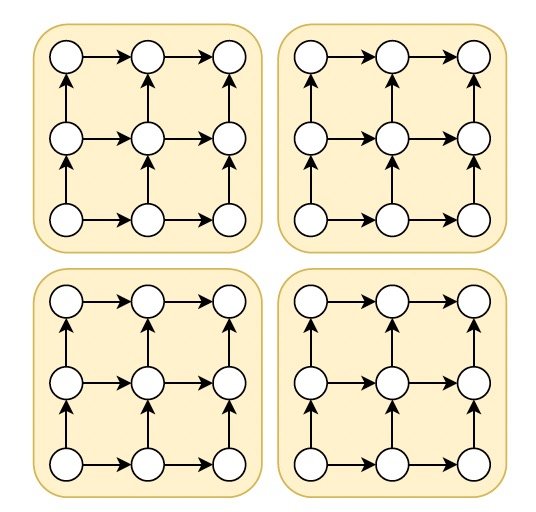
\includegraphics[width=6cm]{fig/pjacobi}
	\caption{分块Jacobi}
	\label{fig:pjacobi}
\end{figure}
\subsubsection{Line Gauss-Seidel}
我们可以将一列的点看成一个整体,这样问题退化为二维的情形,可以对其使用Jacobi迭代,每个格点只更新“侧面”的点,最后再在每一列的内部逐点更新。也可以把每个面看成一个整体,里面的每个点并行更新“侧面”的值,之后每个面内部进行一个二维的G-S迭代。这两种方法都是Jacobi迭代的部分有利于并行,内部的更新无法并行,也都可以利用之前提到的合并残差计算和更新的策略,但由于总体的并行度没有Jacobi或Red\& Black高,(分别约为Jacobi的$1/N$和$1/N^2$)所以效果也较差。
\begin{figure}[H]
	\centering
	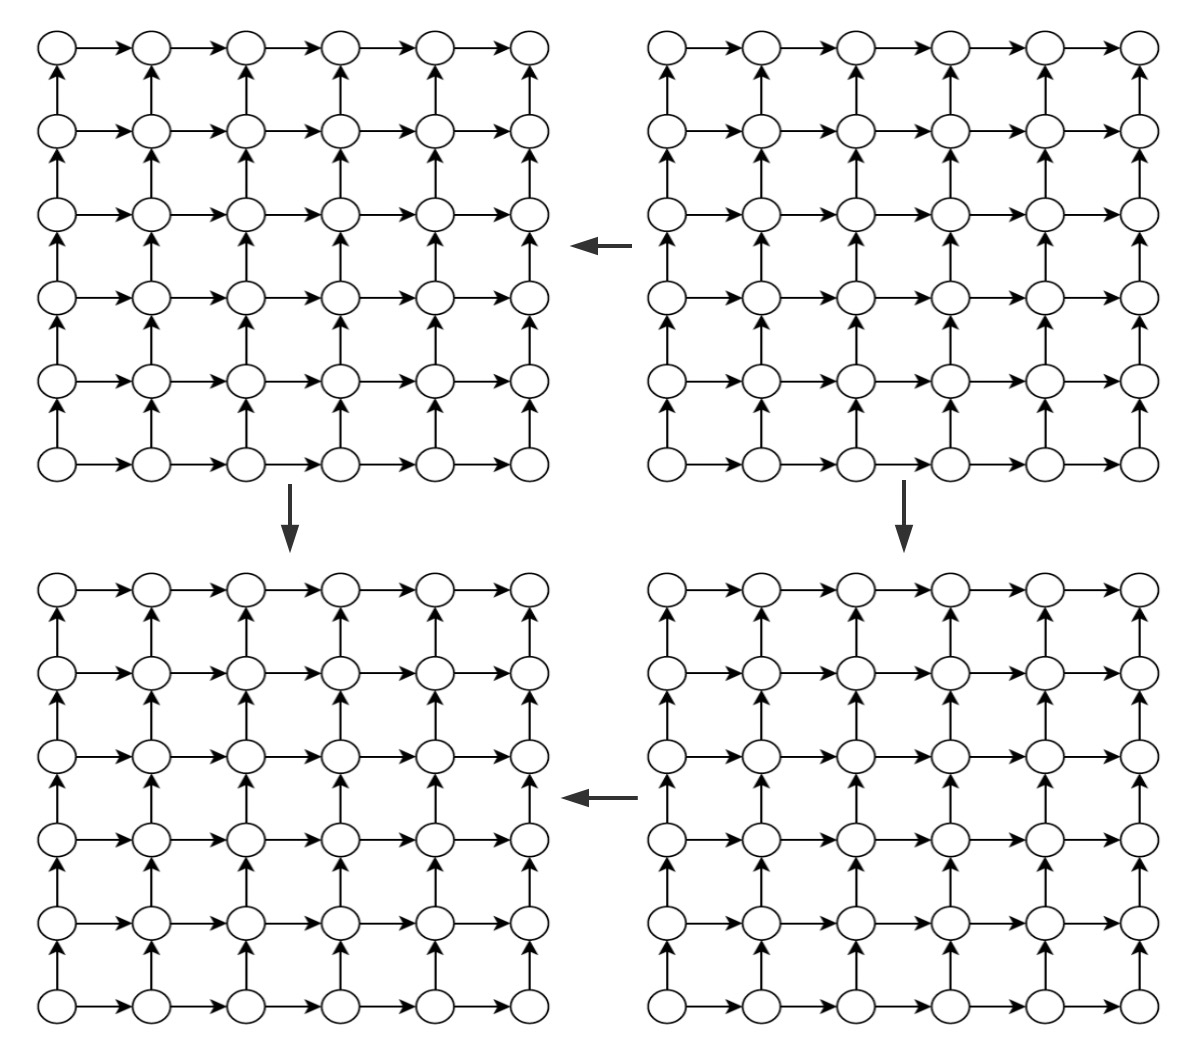
\includegraphics[width=6cm]{./fig/lgs}
	\caption{Line Gauss-Seidel}
\end{figure}
\subsubsection{逐坐标奇偶分类}
与红黑法类似,只是分组不是按照坐标之和,而是按照每个坐标的奇偶性,总共分成8组,每组依次更新,各自使用Jacobi迭代。这样内存访问会比红黑法更不连续,因此需要构造新的更小数组来提高性能。
\section{数值实验}
我们在OpenMP上实现了上面所有的算法,在CUDA上面实现了Jacobi迭代和使用/不使用构造新数组的红黑法,以及 \ref{sec:2.2} 节提到的两种使用共享内存的方式。由于实现OpenMP时发现单CPU多线程计算结果不佳,所以没有使用MPI+OpenMP的方式。出于篇幅限制,我们仅列出在OpenMP,CUDA这两者中各自表现最好的算法用以比较,结果是最好五次运行的中位数。所有的代码和数值结果都可以在./code中找到(请看README中的说明)。
\begin{table}[H]
	\centering
	\begin{tabular}{|c|c|c|c|c|}
	\hline Method & Time (s)& Iter & $\|r\|_2/\|r_0\|$  &  Final residual norm\\ 
	\hline	 Gauss-Seidel(Baseline) & 30.28 &  34 & 9.88e-07 &  7.48e-03 \\
\hline	 Jacobi (OpenMP) & 5.65 &  41 & 5.08e-07 &  3.85e-03 \\
\hline	 R \& B (CUDA) &0.37 & 34 & 1.10e-10 & 8.34e-07 \\\hline
	\end{tabular}
\caption{OpenMP和CUDA中表现最好的算法 (mead of best 5)}
\end{table}
其中R\&B方法的kernel time 约为总时间减去0.001,在迭代过程中仅有传入一个变量$normr$的时间开销。我们选取的OpenMP线程数为8,CUDA的block大小为$4\times1\times 64$,可以看到与我们的分析一致,CUDA上的总时间消耗远远小于OpenMP,且两者都远远好于baseline。我们也可以将Jacobi迭代在OpenMP和CUDA上的表现进行比较。
\begin{table}[H]
	\centering
	\begin{tabular}{|c|c|c|c|c|}
	\hline	Method & Time (s)& Iter & $\|r\|_2/\|r_0\|$  &  Final residual norm \\ 
	\hline	Jacobi (OpenMP) & 5.65 &  41 & 5.08e-07 &  3.85e-03 \\
	\hline	Jacobi (CUDA) &0.53 & 41 & 5.08e-07  &3.85e-03  \\\hline
	\end{tabular}
	\caption{Jacobi迭代在OpenMP和CUDA上的性能比较}
\end{table}
可以看出CUDA上同样的算法了约10倍。此外,我们也可以对Jacobi在CUDA上使用 \ref{sec:2.2} 节提到的两种不同的访存方式进行比较。
\begin{table}[H]
	\centering
	\begin{tabular}{|c|c|c|}
		\hline	Method & Time(s) & Average time of each iteration (s)\\ 
		\hline	直接访存  &0.53 & 0.012 \\
		\hline	共享变量 &0.59 &  0.013\\\hline
	\end{tabular}
	\caption{直接访存全局变量和存储扩展大小的共享变量}
\end{table}
可以看到使用类似于ex5的矩阵乘法那样,预存储共享变量反而速度更慢。主要原因在于,如同 \ref{sec:2.2} 节分析的那样,需要存储比block三个维数各大2的共享变量,由此造成的线程簇分歧和额外的全局变量访问影响了算法的性能,反而使得结果不如直接存取全局变量。

我们再来比较CUDA上Jacobi迭代和两种存储结构R\&B的结果。
\begin{table}[H]
	\centering
	\begin{tabular}{|c|c|c|c|}
		\hline	Method & Time(s) & Average time of each iteration(s) &Average time of resnorm reduce(s)\\ 
		\hline	Jacobi  &0.53 & 0.012 & 2.82e-05\\
		\hline	R\&B(直接访问) &0.56 &  0.016 &1.67e-05\\
		\hline	R\&B(RB分开存) &0.37 &  0.011 &1.67e-05\\\hline
	\end{tabular}
	\caption{CUDA上各算法性能比较}
\end{table}
可以看到在CUDA上的各算法中,没有优化连续地址访存(每次间隔为2)的Red Black单次迭代反而比Jacobi迭代慢,而将Red,Black两种颜色分开存储,访问时可以连续访问的R\&B就显著快于另两种,单次迭代也更快(这也可能是因为不连续地址的间隔由Jacobi的$512,512^2$变为了$256,256*512$的原因)。因此,可以看出在CUDA的计算中,最影响结果的实际上是访存时间,计算时间几乎可以忽略不计。规约用时红黑法约为Jacobi迭代的一半,这也与我们分析的时候,指出我们优化后的算法中,实际上只需要计算一半的残差有关。

最后,我们再来比较OpenMP上比较典型的几个算法的结果。
\begin{table}[H]
	\centering
	\begin{tabular}{|c|c|c|c|c|}
		\hline	Method & Time(s) & Iter & $\|r\|_2/\|r_0\|$  &  Final residual norm \\ 
		\hline	Jacobi  & 5.65 &  41 & 5.08e-07 &  3.85e-03 \\
		\hline	 R\&B & 11.68&  34 & 1.10e-10 & 8.34e-07  \\
		\hline	 part Jacobi &7.92 & 35 & 6.91e-07  &5.12e-03 \\
		\hline	 line G-S &18.10 & 34 & 5.918e-07  &4.47e-03  \\\hline
	\end{tabular}
	\caption{OpenMP上算法性能比较}
\end{table}
可以看到Jacobi迭代具有压倒性的优势,主要是Jacobi的依赖关系使得其可以合并残差计算和更新,这就减少了约一半的时间,此外Jacobi所有的计算都能并行,这也是巨大优势。我们在OpenMP上的红黑法没有实现两色分别存储的格式,其表现出来的性能不如Jacobi,这与CUDA上是一致的。此外,值得一提的是,part Jacobi,即分成8块,块内分别G-S迭代的算法性能反而是第二好的。
\section{总结}
在本次上机作业中,我们通过修改变量之间的依赖关系,改进了Gauss-Seidel迭代,构思了若干用于提高并行度,加快计算速度的迭代格式,对它们进行了理论分析和算法实现。通过理论分析,我们发现了,对于最大活跃线程数高的GPU而言,其计算总时间会远远低于使用几线程或进程的CPU,并且通过数值实验验证了这一点。最终我们通过反复优化访存、计算,达到了接近100倍的加速。至此我们完成了全部的并行与分布式计算基础大作业!
	\bibliographystyle{unsrt}  
	\nocite{*}
\bibliography{ref}
\end{document}